\chapter{State of the Art}
\label{chap:stateofart}

This chapter introduces a modest literature review regarding \gls{IoT}.
Following this two themes some related technologies are briefly presented and then compared.
The intent of this chapter is to introduce the reader to the subjects related to this work.

\section{Internet of Things}
\label{sec:stateofart:iot}

The \gls{IoT} is the collective network of connected devices and technologies that facilitates communication between devices and the cloud. According to \cite{LEE2015431}, it's recognized as one of the most important areas of future technology and is gaining vast attention from a wide range of industries.

It is an essential pillar of the fourth industrial revolution (Industry 4.0). According to \cite{ibm-industry4}, Industry 4.0 is revolutionizing the way companies manufacture, improve and distribute their products. Manufacturers are integrating new technologies, including \gls{IoT}, cloud computing and analytics, AI and machine learning into their production facilities and throughout their operations.
But \gls{IoT} is not only about Industry 4.0, it can be used in several sectors and can improve the overall sustainability of organizations.

Ever since the World Commission on Environment and Development's (1987) "Brundtland report", an increasing societal awareness towards environmental impacts of industrial manufacturing has been observable \parencite{sus}. As such, this compels organizations to invest in this subject, despite its challenges and low rats of success \parencite{iot-fail}.

To better present this topic and its ramifications the following sections will dive into its history, in what contexts it is being used, some of its challenges and renowned solutions.

\subsection{Brief Introduction}
\label{subsec:stateofart:iot:intro}

The \gls{IoT} is a new paradigm that has changed the traditional way of living into a high tech life style. Smart city, smart homes, pollution control, energy saving, smart transportation, smart industries are some of the transformations due to \gls{IoT} (\cite{iot-intro}).

According to \cite{iot-history}, the first literature works about \gls{IoT} are dated 2006. These works, specially, \cite{1581336}, described the environmental benefits one could have using \gls{IoT} technologies.
The case study described in \cite{1581336} revolves around a pilot regarding smart lighting in public roads.
This pilot, implemented in Oslo, generated energy savings of 70\% over the old lights that it replaced.
Nowadays, with the technological advances made, the expected energy savings would be even bigger.

Several other studies, such as \cite{iot-santander}, \cite{iot-barcelona} and \cite{iot-water} further emphasis the benefits \gls{IoT} brings to the table.

\subsection{Business Areas}
\label{subsec:stateofart:iot:areas}

Even though there's no concise structure, it is obvious that the \gls{IoT} technologies can be used in a broad range of areas/sectors. According to \cite{nivzetic2019smart}, the most valuable areas are: Smart Cities, Industrial \gls{IoT}, Connected Health and Smart Homes. The general market division of IoT technologies is presented in Figure~\ref{fig:iot-areas}.

\begin{figure}[H]
    \centering
    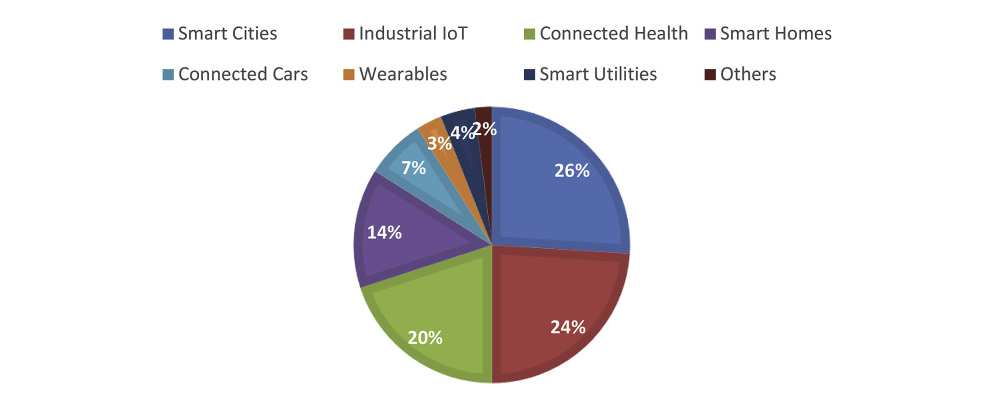
\includegraphics[scale=0.5]{
        assets/figures/iot-areas.png
    }
    \caption[IoT market structure]{General market structure of IoT technologies, \cite{nivzetic2019smart}}
    \label{fig:iot-areas}
\end{figure}

From another point of view, and according to \cite{7073822}, the sectors \gls{IoT} is related to are: Energy, Smart City, Transportation, Smart Home, Environment, Supply Chain, and Health Care.

According to (\cite{6851114}) these are the main application fields for \gls{IoT} in China: industry, smart agriculture, smart logistics, intelligent transportation, smart grids, smart environmental protection, smart safety, smart medical and smart home.

Even though this work focus mostly on Smart Cities other areas will also be described. Each of this areas incorporate several interconnected use cases that will briefly described in the following segments in accordance with \cite{nivzetic2019smart}.

\subsubsection{Smart Cities}
\label{subsubsec:stateofart:iot:areas:cities}

The Smart Cities sector includes numerous use cases related to public safety, the environment, mobility, energy, infrastructure and many other municipal concerns. According to \cite{iot-smart-city-prioritized} this are the use cases being prioritized.

\begin{itemize}
    \item Connected Public Transport: real-time monitoring of public transportation vehicles' locations, stops and itineraries, and the possibility to be notified when a public transportation vehicle is arriving at a stop;
    \item Traffic Monitoring and Management: real-time monitoring and management of traffic flows in a efficient manner;
    \item Water level / Flood Monitoring: real-time monitoring of level of water in public water basins such as rivers, channels, or even lakes and seas to warn and predict fast water level shifts;
    \item Video Surveillance \& Analytics: real-time monitoring using \gls{CCT} cameras and analytics to detect specific situations, e.g. accidents, crimes, potential threats, or recognize specific features (face recognition, demographics, etc.);
    \item Connected Streetlights: real-time monitoring and management of streetlights' health status and energy consumption to decrease costs and become more sustainable;
    \item Weather Monitoring: real-time monitoring of weather conditions such as temperature, humidity, rainfall, wind speed and direction to predict the weather and future natural disasters;
    \item Air Quality / Pollution Monitoring: real-time monitoring of air quality to warn the community about hazardous conditions;
    \item Smart Metering - Water: remote real-time monitoring of water usage in homes to address the world's water demand and scarcity issues and faster localize sewage leaks;
    \item Fire / Smoke Detention: real-time monitoring of possible indoor fires and CO2 levels to prevent injuries, fatalities and building degradation;
    \item Water Quality Monitoring: real-time monitoring of water conditions such as pH levels, percentage of salts and other elements that can threaten the public health.
\end{itemize}

Apart from these use cases, others are arising, such as smart parking (\cite{GOAP201841}), smart irrigation (\cite{7562735}) and waste management (\cite{7972276}).
\begin{itemize}
    \item Smart parking provides a simple method to the community of knowing the available parking spots, which, alone, lowers the carbon footprint and traffic congestions in cities.

    \item Smart irrigation tackles the need to save water by irrigating the soil only when needed and not when it is already moist, it's raining or it is expected to rain in the following hours.

    \item Waste management can eliminate the cost of unnecessary waste collections and therefore reduce the carbon footprint. Data gathered can then help to identifying cost-effective itineraries to collect waste and eventually lower overall transportation and staff costs.
\end{itemize}

All this use cases refine the efficiency of the municipal workforce and help the town council to reduce costs and improve the environment sustainability in the long term.

\subsubsection{Industry}
\label{subsubsec:stateofart:iot:areas:industry}

According to \cite{iiot}, ``the Industrial \gls{IoT} provides a way to get better visibility and insight into the company's operations and assets", therefore this leads to ``operational efficiency gains and accelerated productivity, which results in reduced unplanned downtime and optimized efficiency, and thereby profits"".
It is comprised of several use cases (\cite{iiot-cases}) such as:

\begin{itemize}
    \item Predictive Maintenance: real-time monitoring of equipment conditions and applied data analytics can help a company to significantly decrease operational expenditures. ``Other potential advantages include increased equipment lifetime, increased plant safety and fewer accidents with negative environmental impact"" (\cite{iiot-cases});
    \item Smart metering: real-time monitoring of energy, water or natural gas consumption of a building can reduce operating expenses by managing manual operations remotely, reduce energy theft and improve forecasting and streamline power-consumption (\cite{metering-sierra});
    \item Asset tracking: real-time monitoring of resources helps "to easily locate and monitor key assets, along the supply chain (e.g. raw materials, final products and containers) to optimize logistics, maintain inventory levels, prevent quality issues and detect theft" (\cite{iiot-cases}).
    \item Connected vehicles: computer-enhanced vehicles that automate many normal driving tasks can lower crash rates, and help decreasing the number of vehicles a company needs to function.
    \item Fleet management: real-time monitoring of vehicles location and conditions can help ``improving efficiency and productivity while reducing overall transportation and staff costs"" (\cite{iiot-cases}).
\end{itemize}

As we can see from the list above, the Industrial \gls{IoT} sector is focused on business efficiency and staff safety, which, as a side effect, brings environmental benefits.

\subsubsection{Healthcare}
\label{subsubsec:stateofart:iot:areas:healthcare}

According to \cite{FIROUZI2018583} new opportunities are now arising as a result of fast-paced expansion in the areas of the \gls{IoT} and Big Data for healthcare industries. People across the globe have begun to adopt wearable biosensors, whose data is feed into the new emerging individualized health applications.
This sector incorporates numerous use cases (\cite{iot-healthcare}) such as:

\begin{itemize}
    \item Remote Healthcare Monitoring: real-time monitoring of a patient conditions such as pulse rate and heartbeat can prevent unwanted deaths;
    \item Drug management: medicine monitoring and reminder system can help the elderly to take medicine on time;
    \item Employee health management: real-time monitoring of employee's state can predict burnouts and increase a workforce productivity;
\end{itemize}

The benefits these use cases provide are a more convenient lifestyle, improvement of one life's quality, reduction in costs and increased survival rates of patients (\cite{iot-healthcare}).

\subsubsection{Smart Homes}
\label{subsubsec:stateofart:iot:areas:home}

Visions of smart homes have long caught the attention of researchers and considerable effort has been put toward enabling home automation. However, these technologies have not been widely adopted despite being available for over three decades (\cite{iot-smarthomes}).
Based on \cite{smarthome-review} most home automation services offer the following use cases:

\begin{itemize}
    \item Smart Lighting: remote and automated control of lights inside a house can help to decrease energy wasted;
    \item Smart Air Conditioning: remote and automated control of air conditioners can keep the house comfortable while minimizing the energy wasted;
    \item Remote health monitoring: when dealing with the elderly, complex smart systems can anticipate their needs without direct human intervention;
    \item Device Automation: smart systems can turn the lights off when no one is home, open the door when an identified person arrives and must more, improving the overall comfort of the residents.
\end{itemize}

A smart home delivers various benefits such as reducing energy waste, comfort, allowing remote control of the house, monitoring of elderly patients and easy communication with health institutions (\cite{smarthome-review}).

\subsection{Open Challenges}
\label{subsec:stateofart:iot:challenges}

Even though it seems \gls{IoT} is the obvious next step for the industry, healthcare, everyone's home, public spaces/services and everything else there are some obstacles to overcome.

One of the big challenges ahead of everyone is related with antiquated ideas, tools and processes still in use today.
Each of the use cases above mentioned require a big shift in how a company works since it demands a modernization of the organization infrastructure.
\cite{tapscott2006wikinomics}, explained that ``In an age where mass collaboration can reshape an industry overnight, the old hierarchical ways of organizing work and innovation do not afford the level of agility, creativity, and connectivity that companies require to remain competitive in today's environment"".

According to \cite{7073822} this are the most important challenges regarding \gls{IoT} applications:

\begin{itemize}
    \item Technological Interoperability: achieving a seamless interaction between devices and people with devices (according to \cite{al2016iot} there's a lack of standardization in \gls{IoT} devices and technologies);
    \item Semantic Interoperability: guaranty that the devices interpret the shared information
correctly and act accordingly (improvements have to be made regarding distributed ontologies, semantic web, or semantic device discovery);
    \item Security and Privacy: improving data integrity, unique device identification, encryption and implement proper data/device ownership for legal/liability issues;
    \item Smart Things: ultra low power circuits and devices capable of tolerating harsh environments have to be developed;
    \item Resilience and Reliability: in industrial environments or in emergency use cases temporary outages cannot be accepted.
\end{itemize}

According to the author this challenges substantially lingered the growth of \gls{IoT}, an area that was expected to have a much bigger impact in day-to-day life of everyone. According to \cite{iot-cisco-prediction} there would be 50 billion of devices connected to the Internet by 2020 but \cite{statista-number-devices} reported only 8.74 billion of connected devices.

\cite{noura2019interoperability} introduced more issues in \gls{IoT} related to interoperability from different perspectives:

\begin{itemize}
    \item Device interoperability: concerned with the exchange of information between heterogeneous devices and the ability to integrate new devices into any \gls{IoT} platform;
    \item Network interoperability: concerned with information addressing, routing, security, resource optimization, \gls{QoS} and mobility support;
    \item Syntactical interoperability: concerned with the format and structure of the information exchanged between heterogeneous systems;
    \item Semantic interoperability: concerned with the meaning behind the information exchanged, heterogeneous devices can, for example, work with diverse unit measurements;
    \item Platform interoperability: concerned with heterogeneous platforms that use diverse programming languages, \gls{OS} and software architectures.
\end{itemize}

For \gls{IoT} Technologies to deliver on the promises made by companies like Cisco or Gartner, these barriers must be surpassed.

\subsection{Renowned Solutions}
\label{subsec:stateofart:iot:solutions}

According to \cite{iot-platforms} there were more than 300 \gls{IoT} platforms in the 2016 market. This section will briefly review some of the most impactful platforms.

The first three reviewed platforms are part of major cloud computing services such as Azure, AWS and Google Cloud, and will be evaluated with the help of \cite{pierleoni2019amazon}.
The Things Network is an open-source solution that can be compare to the previously three solutions in terms of functionalities.
DataCake is a \gls{SaaS} solution with a low-code component to build applications.
Verizon Connect is a full-fledged Fleet Management \gls{SaaS} solution.

\subsubsection{Azure IoT}
\label{subsubsec:stateofart:iot:solutions:azure}

Azure IoT refers to a collection of managed and platform services across edge and cloud that connect, monitor, and control billions of IoT assets (\cite{azure-iot}). According to \cite{pierleoni2019amazon} this platform provides two paths: a \gls{PaaS} solution, and a \gls{SaaS} solution.

Regardless of the path chosen each solution is composed by multiple Azure services, like Azure IoT Hub, Azure IoT Central, Azure Data Lake, Azure Data Bricks, Event Hub, Database Services, Azure Function and many more.

 The \gls{PaaS} solution enables the creation of the needed solution using any azure services that can be configured to behave together.

The \gls{SaaS} solution has four big areas, Retail, Energy, Healthcare and Government. Each of this areas contain several solutions.

This are the solutions provided by each Azure IoT area:

\begin{itemize}
    \item Retail: Connected logistics, Digital distribution center, In-store analytics - condition monitoring, In-store analytics - checkout, Smart inventory management, Micro-fulfillment center;
    \item Energy: Smart meter monitoring, Solar panel monitoring;
    \item Healthcare: Continuous patient monitoring;
    \item Government: Connected waste management, Water consumption monitoring, Water quality monitoring;
\end{itemize}

\subsubsection{AWS IoT Core}
\label{subsubsec:stateofart:iot:solutions:aws}

AWS IoT Core can be seen as a \gls{PaaS} solution that allows for device management, uses rules to interact with other AWS services and allows for data storage. Communication between the platform and the devices is made using \gls{MQTT} topics (\cite{pierleoni2019amazon}).

This platform does not provide any pre-made solution leaving that burden for each client.

\subsubsection{Google IoT Cloud}
\label{subsubsec:stateofart:iot:solutions:google}

Google IoT Cloud is also a \gls{PaaS} solution with much of the feature provided by AWS IoT Core, it also doesn't support pre-made solutions. According to \cite{pierleoni2019amazon}, it is possible to define custom metadata for a device with an arbitrary user-defined blob of data, something that Azure and AWS don't support.

\subsubsection{The Things Network}
\label{subsubsec:stateofart:iot:solutions:ttn}

The Things Network is a solution to handle device management and applications that will use the information provided by this devices (\cite{ttn}). This solution comes with various subscription plans but is based on a open-source license. The code is publicly available and can be used without any subscription. It distinguishes it self from the previously platforms since it can be used on-premise and with no extra costs. It doesn't support any pre-made solutions, that responsibility is tied to the "applications" mentioned before.

\subsubsection{DataCake}
\label{subsubsec:stateofart:iot:solutions:datacake}

DataCake is a multi-purpose, low-code \gls{IoT} platform that requires no programming skills and minimal time to create custom \gls{IoT} applications that can be brought into a white label \gls{IoT} solution at the push of a button (\cite{datacake}).

It provides several pre-made solutions like Welding Fume Monitoring, Urban Air Quality,Industrial Gas Supply, Air Quality Monitoring, Climate Monitoring, Cryogenics Monitoring, CO2 Monitoring, Water Level and Flood Monitoring and Industrial \gls{IoT}.

\subsubsection{Verizon Connect}
\label{subsubsec:stateofart:iot:solutions:verizon}

Verizon Connect is a Fleet Management solution that provides it's own sensors/devices, platform and application under a subscription (\cite{verizon-iot}).
A team from Verizon installs the devices in the fleet according to specification and access to the platform is given. This is an Hassle-free solution but the costs associated with it can be high.

\subsubsection{Synopsis}
\label{subsec:stateofart:iot:solutions:synopsis}

The intent behind the election of this specific solutions derive from the need to clarify what the market is currently lacking.
This solutions can be grouped into 4 groups:

\begin{itemize}
    \item Solutions with no pre-made applications (AWS IoT Core, Google IoT Cloud, The Things Network and partially Azure IoT);
    \item Solutions with a single pre-made application (Verizon Connect, JDLink, Ericsson Maritime ICT and many, many more);
    \item Solutions with various pre-made applications (DataCake and Azure IoT);
    \item Solutions that provide a simple manner to build custom applications (DataCake);
\end{itemize}

In a continuous evolving environment like \gls{IoT} is, there is no easy way for a company to encompass various solutions without subscribing to various services that aren't interoperable.

The only solutions that provide this are Azure IoT and DataCake.
Sadly, none of this solutions provide an on-premise license and both lack various use cases.

\section{Related Technology}
\label{sec:stateofart:tech}

This section focus on concepts that try to answer the problems related to \gls{IoT} and Big Data.
This concepts are Asynchronous Communication, Data Processing and Data Storage.
For each concept some relevant technologies will be briefly presented and then compared.

\subsection{Asynchronous Communication}
\label{subsec:stateofart:tech:async}

Asynchronous Communication is a one-way communication between two or more entities usually though a message broker.

"Distributed Message Brokers are typically used to decouple separate stages of a software architecture. They permit communication between these stages asynchronously, by using the publish-subscribe paradigm" (\cite{john2017survey}).

The two message broker that will be presented are Kafka (\cite{kafka}) and RabbitMQ (\cite{rabbitmq}).

\subsubsection{Kafka}
\label{subsubsec:stateofart:tech:async:kafka}

Kafka is an open source distributed event streaming platform designed to handle high throughput.
According to \cite{goodhope2012building} Kafka was originally built at LinkedIn as its centralized event pipelining platform and later open sourced.

Kafka main components are producers, topics and consumers. The message brokering task is handled by topics, that producers write to and consumers read from.

\subsubsection{RabbitMQ}
\label{subsubsec:stateofart:tech:async:rabbitmq}

RabbitMQ is an open source message broker that supports various protocols such as \gls{AMQP} and \gls{MQTT}, it was built at Rabbit Technologies Ltd. and later open sourced (\cite{rabbitmq}).

"RabbitMQ takes a modular approach, dividing the message brokering task between exchanges and message queues" (\cite{10.1145/3093742.3093908}).
According to \cite{rabbitmq} producers write to exchanges and consumers read from queues.

\subsubsection{Comparison}
\label{subsubsec:stateofart:tech:async:comp}

A brief comparison of this two technologies, Kafka and RabbitMQ, is presented according to \cite{john2017survey}, \cite{10.1145/3093742.3093908} in the Table~\ref{tab:async}.

\begin{table}[H]
\renewcommand{\arraystretch}{1.4}
\caption{Comparison of Asynchronous Communication Technologies}
\label{tab:async}
    \centering
    \begin{tabular}{m{9em} m{12em} m{12em} }
    \toprule
\tabhead{Technology} & \tabhead{Kafka} & \tabhead{RabbitMQ} \\
        \midrule
        Support \gls{AMQP} & Only through plugins, Kafka has its own protocol & Native \\
        Support \gls{MQTT} & Only through plugins & Only though plugins \\
        Message Routing & No complex routing, messages are sent to brokers & Complex routing, messages are sent to exchanges that have queues bind to them \\
        Message Persistence & Writes to a persistent file system & A configuration option while creating a queue \\
        Message Batching & Native & Though RabbitMQ Stream \\
        Message Reliability & No acknowledgement is sent & Receiver sends acknowledgement \\
        Message Distribution Medium & Topic & Queue \\
        Message Format & Bytes, easier to develop for & Binary, better compression \\
        Support Kubernetes Deployment & Though "Kafka Operators" & Though "RabbitMQ Cluster Kubernetes Operator" \\
        Ease Of Use & High & High \\
        \bottomrule\\
    \end{tabular}
\end{table}

\subsection{Data Processing}
\label{subsec:stateofart:tech:process}

Data Processing is a complex topic at the core of Big Data. To better deal with this needs several streaming processing frameworks have been develop. "Stream processing problems lead to several research questions such as how to design scalable environments, how to provide fault tolerance and how to design efficient solutions" (\cite{inoubli2018comparative}).
According to \cite{isah2019survey} the key features of this frameworks are: (i) programming model, (ii) data source interaction model, (iii) data partitioning strategy, (iv) state management, (v) message processing guarantee, (vi) fault tolerance and recovery, (vii) deployment, and  (viii) support base (e.g. community, high level language, advanced input sources, storage, and analytics).

Three streaming processing frameworks will be presented: Spark (\cite{spark}), Flink (\cite{flink}), and Storm (\cite{storm}).

\subsubsection{Spark}
\label{subsubsec:stateofart:tech:process:spark}

"Apache Spark  is a powerful processing framework that provides an ease of use tool for efficient analytics of heterogeneous data" and "In Spark, there are two types of operations on Resilient Distributed Datasets: transformations and actions" (\cite{inoubli2018comparative}).

\subsubsection{Flink}
\label{subsubsec:stateofart:tech:process:flink}

"Flink is a hybrid processing platform, supporting both stream and batch processing. Flink core is the stream processing, making batch processing a special class of application. Analytics jobs in Flink compile into a directed graph of tasks" (\cite{lopez2016performance}).
"The programming model of Flink is similar to MapReduce. By contrast to MapReduce, Flink offers additional high level functions such as join, filter and aggregation" (\cite{inoubli2018comparative}).

\subsubsection{Storm}
\label{subsubsec:stateofart:tech:process:storm}

"Storm is an open source framework for processing large structured and unstructured data in real time. Storm is a fault tolerant framework that is suitable for real time data analysis, machine learning, sequential and iterative computation" (\cite{inoubli2018comparative}).
Storm defined two main abstract concepts to handle data, spouts (entry points) and bolts (functions that transform data).

\subsubsection{Comparison}
\label{subsubsec:stateofart:tech:process:comp}

A brief comparison of this three technologies, Spark, Flink and Storm, is presented according to \cite{lopez2016performance}, \cite{wingerath2016real}, \cite{isah2019survey}, \cite{inoubli2018comparative} in the Table~\ref{tab:stream}.

\begin{table}[H]
\renewcommand{\arraystretch}{1.4}
\caption{Comparison of Data Processing Frameworks}
\label{tab:stream}
    \centering
    \begin{tabular}{m{5em} m{9em} m{9em} m{9em}}
    \toprule
        \tabhead{Technology} & \tabhead{Spark} & \tabhead{Flink} & \tabhead{Storm} \\
        \midrule
        Processing Model & Micro-batch (Though Spark Streaming) & One-at-a-time & One-at-a-time \\
        Support for Event Time processing & Yes & Yes & No \\
        Lambda Architecture Support & Yes & Yes & No \\
        Fault Tolerant & Yes & Yes & Yes \\
        Latency & Few Seconds & Sub-Second & Sub-Second \\
        Programming Language & Java/Scala & Java/Scala & Java/Closure \\
        Message semantics & Exactly One & Exactly One & At least One \\
        Support Kubernetes Deployment & Though "Spark Operator" & Though "Kubernetes Native" & By replicating storm architecture in K8s with ZooKeeper, Storm master and Storm Workers \\
        API & Declarative & Declarative & Compositional \\
        Ease of Use & Low & Medium & Medium \\
        \bottomrule\\
    \end{tabular}
\end{table}

\subsection{Data Storage}
\label{subsec:stateofart:tech:storage}

Data Storage is at the core of Big Data. There is a high need to efficiently store the huge volumes of data generated everyday, as explained by \cite{6567202}. The industry has evolved a lot in the past and there are solutions that promise to solve this problem.

Three databases will be presented: HBase (\cite{hbase}), MongoDB (\cite{mongodb}), and QuestDB (\cite{questdb}).

\subsubsection{HBase}
\label{subsubsec:stateofart:tech:storage:hbase}

According to \cite{george2011hbase} HBase is a distributed, persistent, strictly consistent storage system with near-optimal write and excellent read performance. This database uses \gls{HDFS} as its file system and so sits on top of Hadoop.
HBase does not support a structured query language like SQL, ``even though it's comprised of a set of standard tables with rows and columns, much like a traditional database"" \parencite{ibm-hbase}. These table must have a primary key that is used to access the each row according to \cite{ibm-hbase}.

\subsubsection{MongoDB}
\label{subsubsec:stateofart:tech:storage:mongodb}

MongoDB is a NoSQL Database. According to \cite{moniruzzaman2013nosql} ``NoSQL systems are distributed, non-relational databases designed for large-scale data storage and for massively-parallel data processing across a large number of commodity servers"".
According to \cite{ibm-mongo,} "as a NoSQL solution, MongoDB does not require a relational database management system (RDBMS), so it provides an elastic data storage model that enables users to store and query multivariate data types with ease".

\subsubsection{QuestDB}
\label{subsubsec:stateofart:tech:storage:questdb}

QuestDB is is a relational column-oriented database designed for time series and event data and entitles it self as the ``fastest open source time series database"" (\cite{questdb}).
According to benchmarks (\cite{quest-bench}) preformed using the \gls{TSBS}, \cite{TSBS}, QuestDB ranks as the fastest option in the market.

\subsubsection{Comparison}
\label{subsubsec:stateofart:tech:storage:comp}

A brief comparison of this three technologies, HBase, MongoDB, QuestDB, is presented in the Table~\ref{tab:stateofart:tech:storage:comp:comp}. This comparisons are based on articles written by \cite{george2011hbase}, \cite{moniruzzaman2013nosql} and \cite{davoudian2018survey} and the \cite{questdb} website.

\begin{table}[H]
    \centering
    \caption{Comparison of Data Storage Technologies}
    \label{tab:stateofart:tech:storage:comp:comp}
    \begin{tabular}{@{}llll@{}}
    \toprule
    \textbf{Technology}      & \textbf{HBase}         & \textbf{MongoDB}            & \textbf{QuestDB}            \\ \midrule
    Cluster Support          & Yes                    & Yes                         & No                          \\
    Storage model            & Wide-column            & Document                    & Column-Based                \\
    Support for Time Series  & Yes                    & Yes, partially              & Yes                         \\
    Relational Database      & No                     & No                          & Yes                         \\
    Support for standard SQL & Through Apache Phoenix & No                          & Yes                         \\
    Data Storage             & HDFS                   & VMFS                        & VMFS                        \\
    Ease of Use              & Low                    & High                        & High                        \\ \bottomrule
    \end{tabular}
\end{table}

\section{Synopsis}
\label{sec:stateofart:synopsis}

This chapter presented the big theme surrounding this work: \gls{IoT}.

In the \gls{IoT} section some business cases relevant for this work were introduced. Besides these, several solutions currently in the market were presented.
The technologies usually used to tackle the challenges related to \gls{IoT} were presented in the \nameref{sec:stateofart:tech} section, these were: (i) Asynchronous Communication, (ii) Data Processing and (iii) Data Storage.

In the following chapter, \nameref{chap:requirements}, some of the business cases and challenges discussed here will be tackled.
